\newchapter{phaseMons}{Phase Monitor Performance}

This is the introductory text.

Mon1 = first mon in CT
Mon2 = second mon in CT
Mon3 = mon in TBL

Mon1/Mon2 = upstream phase
Mon3 = downstream phase

\newsection{monElectronics}{Phase Monitor Electronics}

Hybrid - remove dipole (position dependent) mode. 19dB below monopole mode for 1mm offset (11\% amplitude). 1mm beam offset = 2.8 degrees phase offset. 180 degree hybrids to remove. Additional 20 dB attenuation in dipole mode.

Bunch length sensitivity: more sensitive to variation in bunch length for longer variations. 5mm bunch length - 50\% amplitude output compared to 0mm. With 1mm bunches 16\% variation in bunch length needed to cause 1\% change in output voltage.

LO should have 5fs stability? What is the source of the LO?

Mixer output
\begin{align}
RF(t) &= A_{RF}(t)\cos[\omega_{RF} t + \phi(t)] \\
LO(t) &= A_{LO}\cos[\omega_{LO} t]
\end{align}
mixer multiplies
\begin{align}
\mathrm{Mixer}(t) &= RF(t) \times LO(t) \\
\mathrm{Mixer}(t) &= A_{RF}(t)A_{LO}\cos[\omega_{RF} t + \phi(t)]\cos[\omega_{LO} t]
\end{align}
trig identities
\begin{equation}
\mathrm{Mixer}(t) = \frac{A_{RF}(t)A_{LO}}{2}\left\lbrace\cos[(\omega_{LO} + \omega_{RF})t + \phi(t)] + \cos[(\omega_{LO} - \omega_{RF})t + \phi(t)]\right\rbrace
\end{equation}
filter high frequency
\begin{equation}
\mathrm{Mixer}(t) = \frac{A_{RF}(t)A_{LO}}{2}\cos[(\omega_{LO} - \omega_{RF})t + \phi(t)]
\label{e:mixOutAnyFreq} 
\end{equation}
LO frequency and RF frequency are the same
\begin{equation}
\mathrm{Mixer}(t) = \frac{A_{RF}(t)A_{LO}}{2}\cos[\phi(t)]
\label{e:mixOutSameFreq} 
\end{equation}
Diode used to measure \(A_{RF}\)
\begin{equation}
\mathrm{Diode}(t) = A_{RF}(t)^2
\label{e:idealDiode}
\end{equation}
The phase can be reconstructed by
\begin{align}
&\frac{\mathrm{Mixer}(t)}{\sqrt{\mathrm{Diode}(t)}} = A\cos[\phi(t)] \label{e:mixOverSqrtDio} \\
&\phi(t) = \arccos\left[\frac{\mathrm{Mixer(t)}}{A\sqrt{\mathrm{Diode(t)}}}\right]
\label{e:phaseRecIdeal} 
\end{align}

Beam/monitor frequency is 11.994 GHz.

Performance limited by:
Device non-linearity -- normally better for lower input power
Signal to noise -- better for high power
Therefore, split signal to 8 mixers -- low input power to each one -- to reduce effect of non-linearities. Then sum up results of each mixer to improve signal to noise.

Monitor -> attenuator? -> Hybrid sum -> attenuator? -> attenuator in gallery -> mixer RF input
LO -> phase shifter -> multiplier -> amplifier -> mixer LO input
Mixer output -> attenuator -> amplifier -> SiS OR -> attenuator->FONT
Diode output -> SiS/FONT

Latest power measurements:
Mon1 24.6 dBm + 3dB
Mon2 26.8 dBm + 3dB
Mon3 24.5 dBm
LO1 22.6 dBm
LO2 23.6 dBm
LO3 25.5 dBm

\newsection{sinFitAlgorithm}{Fitting Method}

Due to the dependence of the mixer output on \(\cos(\phi)\) as seen in the previous section, many of the measurements in this chapter require a sinusoidal fit of the form:
\begin{equation}
y = A\sin(bx + c) + d
\label{e:generalSinEq}
\end{equation}
The use of sine rather than cosine makes no difference to the fitted amplitude, \(A\), and offset, \(d\) which are usually the only parameters of interest in this chapter. It is also convenient to consider a mixer output of zero to correspond to zero phase (rather than \(90^\circ\) as in Equation~\ref{e:mixOverSqrtDio}). All the fits of this type have been performed using a weighted nonlinear least squares fit implemented in MatLab fitting libraries \cite{MatLabFit}. Each data point is weighted by the inverse of its standard error squared.

Care must be taken to select suitable initial values for the four parameters in the fit in order to avoid local minima and ensure a reasonable fit. This is particularly important for a sinusoidal fit as there are many solutions with different frequencies and phase offsets that can match the data. The frequency, \(b\), is the most critical parameter but for all the applications in this chapter this is already known, e.g. from the properties of the used phase shifters. Initial values for the three reamining parametrs are estimated as follows:
\begin{align}
A &= \frac{\mathrm{max}(y)-\mathrm{min}(y)}{2} \\
d &= \frac{\mathrm{max}(y)+\mathrm{min}(y)}{2} \\
c &= \arcsin\left(\frac{y-d}{A}\right) - bx
\end{align}
The initial amplitude, \(A\), and offset, \(d\), of the sine curve are simply determined by comparing the minimum and maximum output. These initial estimates are therefore highly biased by any large outliers around the minimum and maximum output, but this is rarely the case for the application here and these simple estimators are sufficient.
Rearranging Equation~\ref{e:generalSinEq} gives the expression for \(c\) above. Due to its use of arcsin the equation is only valid in the first and fourth quadrants, between \(-\pi/2\) and \(+\pi/2\) where the gradient of the sine curve is positive. The \(y\) value at each data point is compared to its neighbours to determine whether it is on the rising slope. The initial value of \(c\) is the mean value calculated across all the data points that meet this criteria.

Figure~\ref{f:sinFitEx} and Table~\ref{t:sinFitEx} show the results of an example fit using this approach. An initial distribution of points with \(y=\sin(x+1)+1\) is used (\(A = b = c = d = 1\)), with random noise added. \(b\) is assumed to be known, as is normal. The initial estimates for \(A\) and \(d\) are within a few percent of their true value. The initial estimate for \(c\) is within \(20\%\) of the correct value. After fitting all four parameters are in agreement with the expected values within error bars.

\begin{figure}
  \centering
  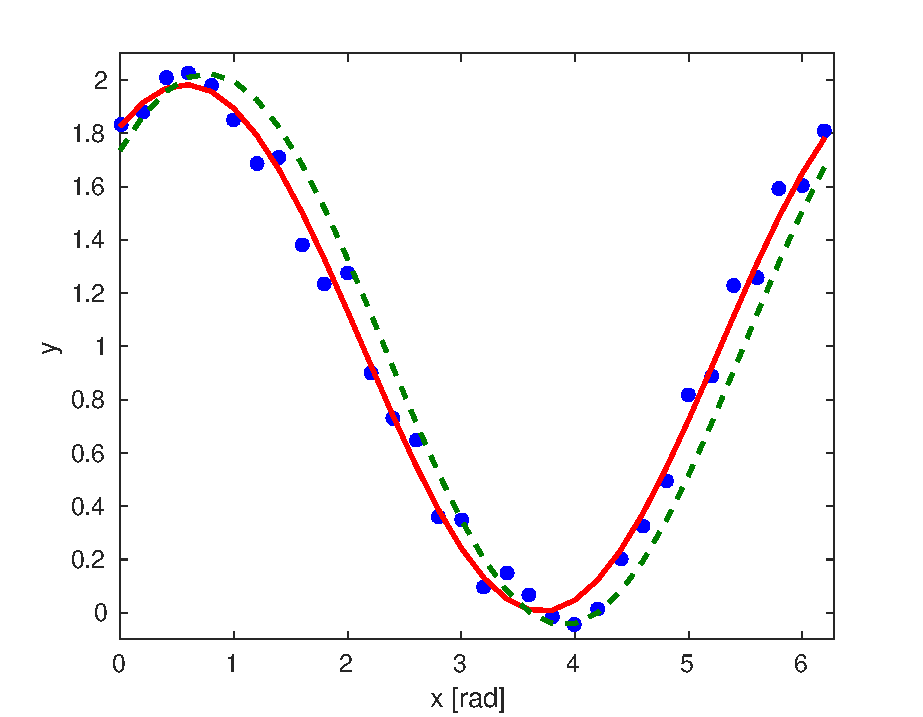
\includegraphics[width=0.9\textwidth]{Figures/phaseMons/sinFitEx}
  \caption{Example sine fit to generated data with added random noise.}
  \label{f:sinFitEx}
\end{figure}

\begin{table}
  \begin{center}
    \begin{tabular}{|c c c c|}
	   \hline
       Parameter & Value & Initial & Fit \\ \hline
       \(A\) & 1 & 1.03 & \(0.99\pm0.02\)\\
       \(b\) & 1 & 1 & \(1.00\pm0.02\) \\
       \(c\) & 1 & 0.81 & \(1.00\pm0.06\) \\
       \(d\) & 1 & 0.99 & \(0.99\pm0.02\) \\ \hline
    \end{tabular}
    \caption{Typical upstream phase and energy conditions at CTF3.}
  	\label{t:sinFitEx}
  \end{center}
\end{table}

\newsection{monSigResponse}{Signal Generator Measurements}

Measurements have been taken using a 12~GHz signal generator to determine the performance of the three sets of phase monitor electronics independently from the phase monitors themselves. In particular, these tests were focused on identifying the saturation and cross-talk characteristics of the output mixer and diode signals in order to determine a suitable input power range to use during normal operation.

\subsection{Experimental Setup}
\label{ss:sigGenSetup}

Two changes were made to the setup shown in Figure~[REF] for these tests. Firstly, the beam induced signal from the phase monitors usually connected to the RF port of the mixers is replaced by the output from a 12~GHz signal generator. To be able to reach the same input power levels as the beam signals the signal generator output is amplified using a [TODO:amplifierInfo]. This allows the input power to the mixers to be varied in a wide range between 0 and 33dBm, or between 0.2 and 10.0~V in terms of voltage. The precise power sent to the mixer is verified between each measurement using a power meter. 

Secondly, the diode outputs were amplified during these tests (using the same amplifier introduced in Section~\ref{ss:sisNoise}) by a factor 10 in voltage to reduce digitiser noise in the measurement. The non-amplified peak diode output is therefore 170~mV, rather than the 1.7~V seen in the plots in this section. The \(\pm500\)~mV mixer outputs have not been amplified. Usually the mixer output is amplified and the diode not amplified, as in Figure~[REF], for reasons that will become clear later in this chapter.

There are some differences between the properties of the generated signal and the beam signal that would be used in normal operation. Firstly, unlike the pulsed beam signal the used generated signal is continuous. It has been verified that the response of the mixers is equivalent for both the continuous and pulsed signals, at least in terms of output power and saturation levels [REF]. The cross-talk properties are difficult to characterise with beam based measurements alone, but assumed to be similar.

Secondly, the phase of the generated signal does not vary with time, compared to the beam signal which has a large \(\sim40^\circ\) phase sag along the pulse and much larger phase jitter. If the signal generator was used at the same frequency as the beam and LO signals, 11.994~GHz, the mixer output would therefore be constant as it depends only on the static phase as per Equation~\ref{e:mixOutSameFreq}. Instead, a generated signal with a slightly lower frequency of 11.991~GHz has been used. From Equation~\ref{e:mixOutAnyFreq} it can be seeen that in this case the mixer output voltage is sinusoidal, with a frequency equal to the frequency difference between the LO and RF inputs -- or \(11.994-11.991\)~GHz = 3~MHz with the setup used here. This has the benefit of being able to see the response of the electronics to all input phases in one measurement, rather than having to take multiple measurements varying the LO phase shifter between each one.

\subsection{Results}
\label{ss:sigGenResults}

Figures~\ref{f:sigGenAllMix1}--\ref{f:sigGenAllDio3} show the mixer and diode outputs for all three sets of electronics at each of the input power levels sent from the signal generator. These will be referred back to and discussed in more detail in the remainder of this section. Some initial observations that are immediately clear from these figures are as follows. All mixer outputs show a sinusoidal oscillation with a frequency of 3~MHz, or 60 samples at the sampling frequency of 192~MHz, as expected. An oscillation with the same frequency is also visible on the diode outputs, with the largest amplitude for the 2nd set of electronics. This is the first hint of the non-ideal characteristics of the diodes. Finally, output of the mixer and diode increases with the input power, as expected. At high input powers the outputs begin to saturate. This is apparent by observing the diode signals, on which the output is much flatter at the highest power levels, without the oscillation seen at low input powers. The characteristics of the mixers are discussed in Section~\ref{ss:sigGenMixer} and the diodes in Section~\ref{ss:sigGenDiode}.

\begin{figure}
  \centering
  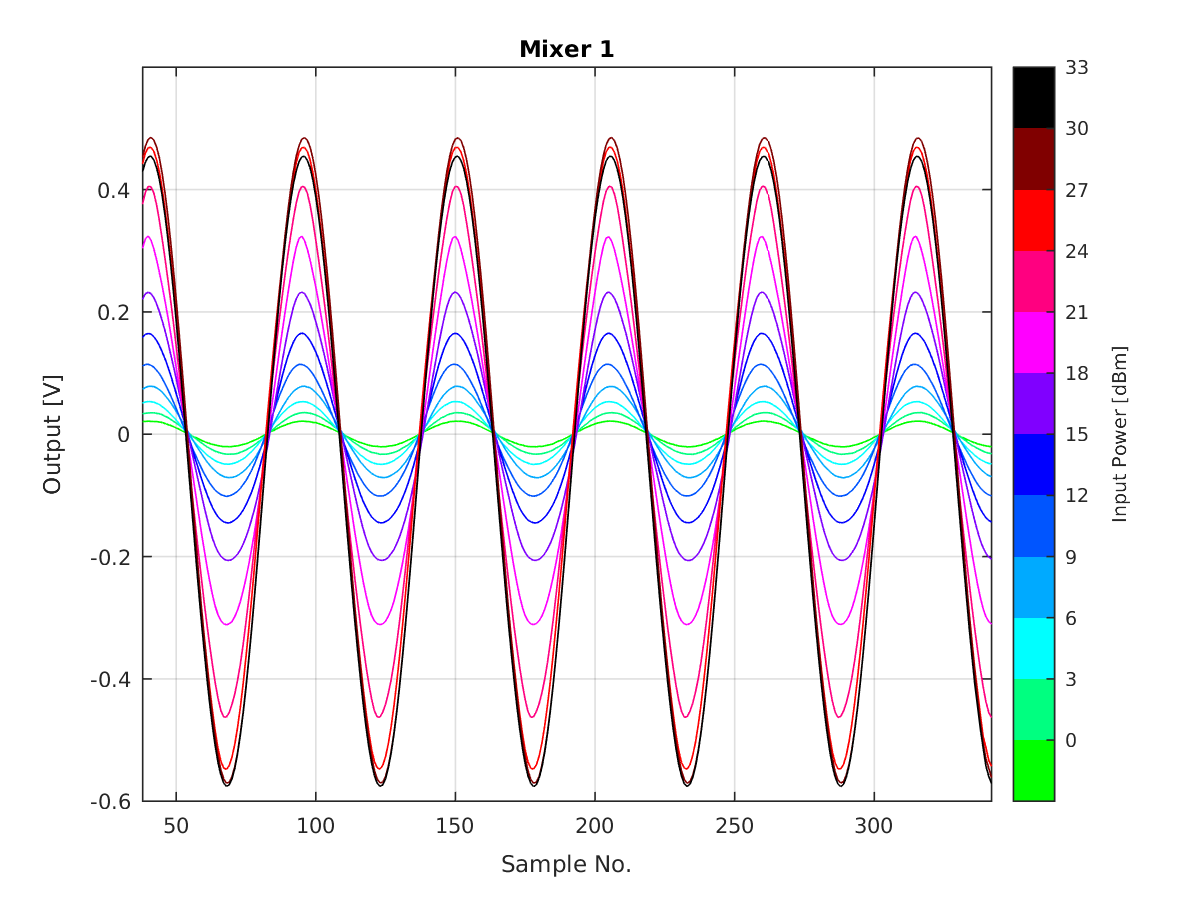
\includegraphics[width=0.9\textwidth]{Figures/phaseMons/Mixer1_AllPowerLevels}
  \caption{Response of Mixer 1 to signal generator input.}
  \label{f:sigGenAllMix1}
  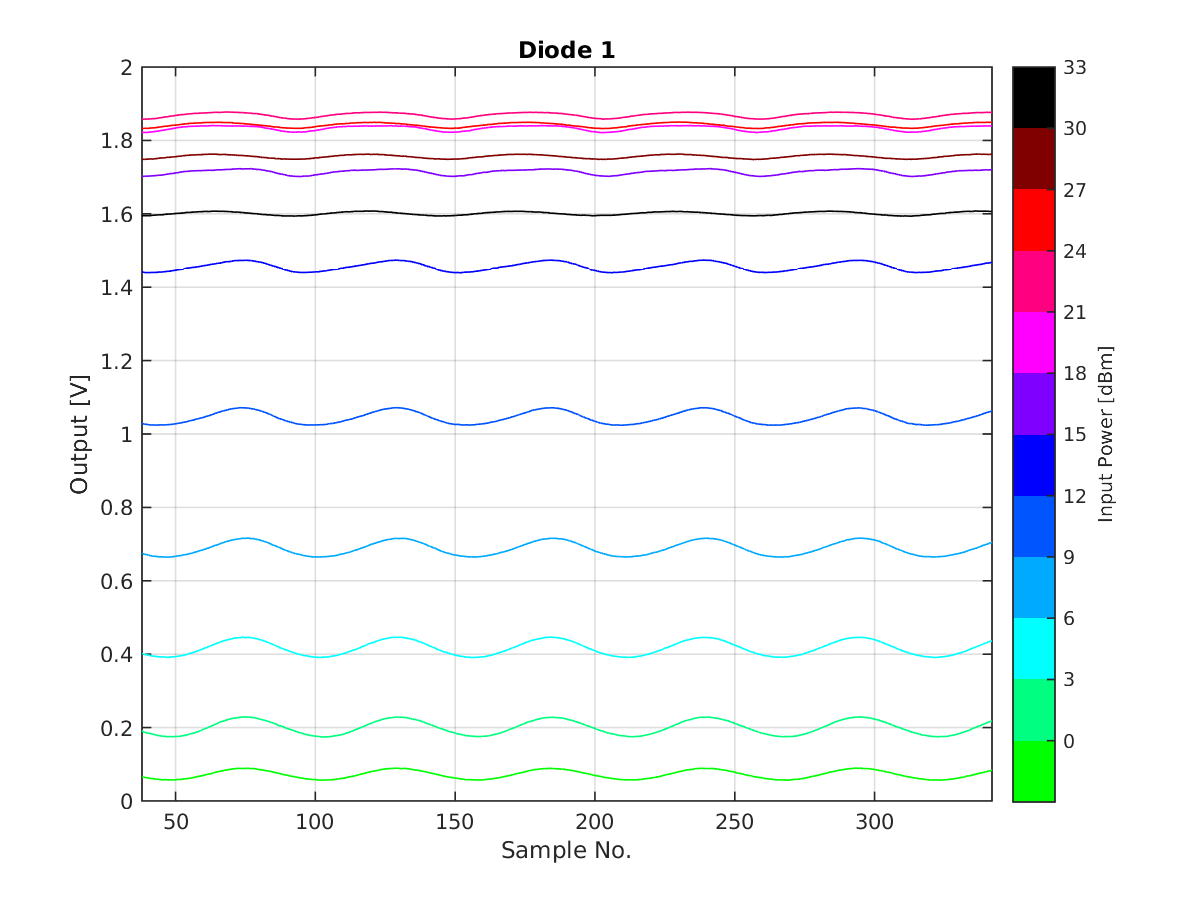
\includegraphics[width=0.9\textwidth]{Figures/phaseMons/Diode1_AllPowerLevels}
  \caption{Response of Diode 1 to signal generator input.}
  \label{f:sigGenAllDio1}
\end{figure}

\begin{figure}
  \centering
  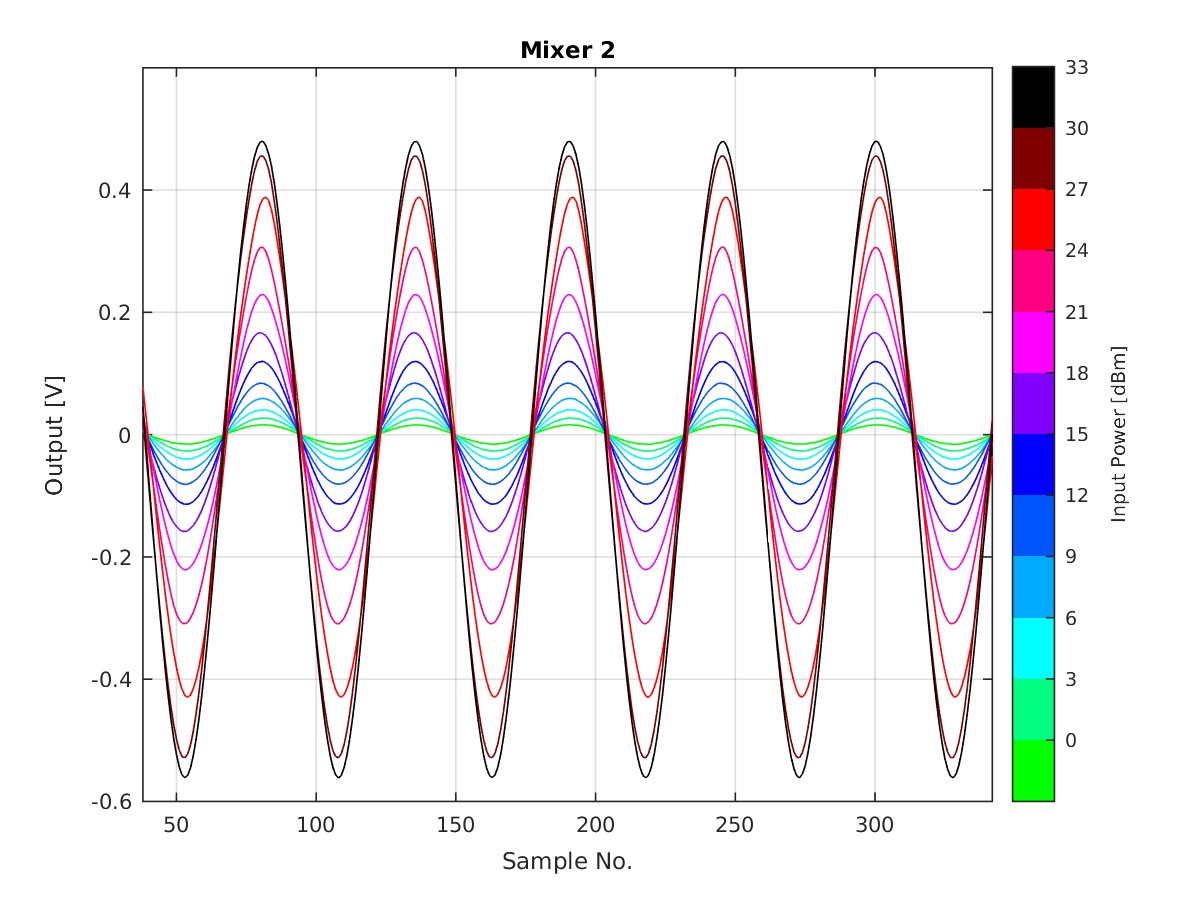
\includegraphics[width=0.9\textwidth]{Figures/phaseMons/Mixer2_AllPowerLevels}
  \caption{Response of Mixer 2 to signal generator input.}
  \label{f:sigGenAllMix2}
  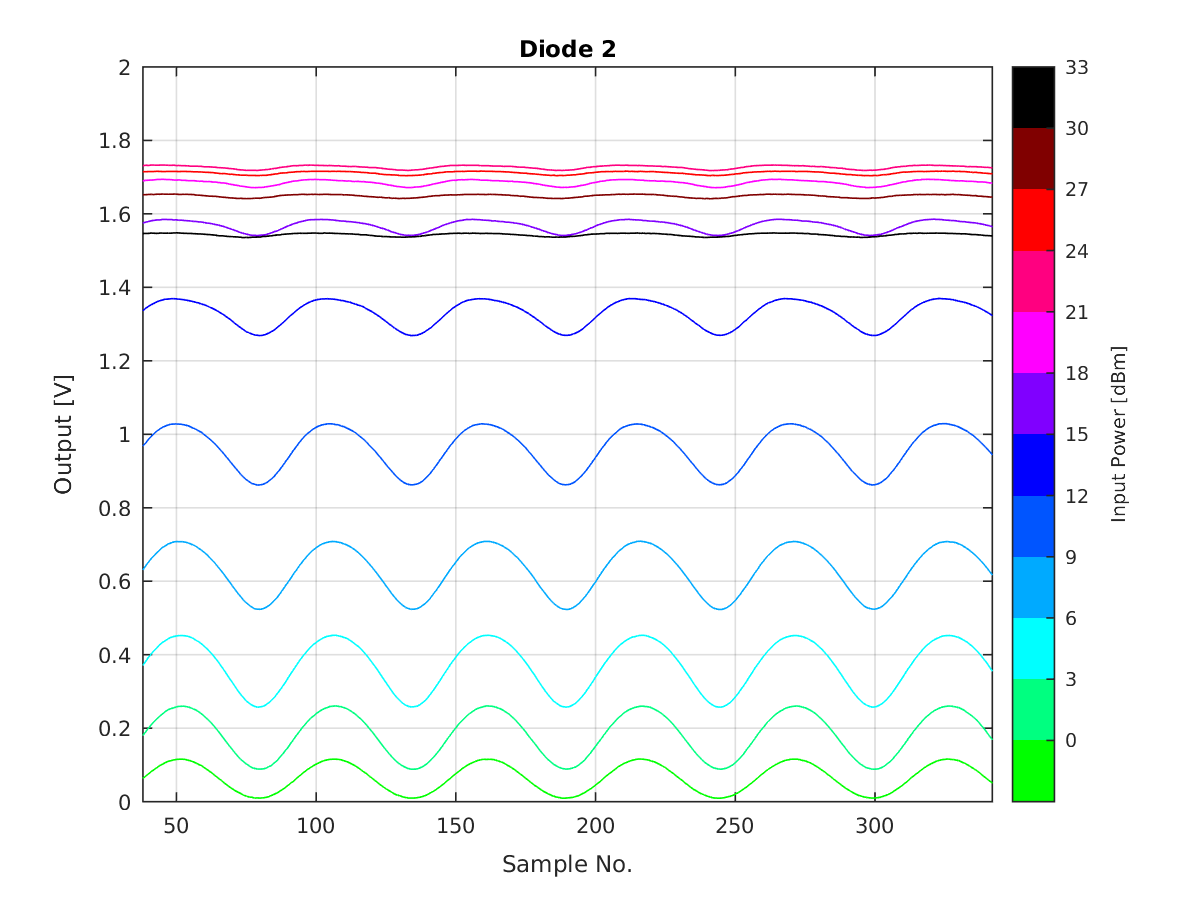
\includegraphics[width=0.9\textwidth]{Figures/phaseMons/Diode2_AllPowerLevels}
  \caption{Response of Diode 2 to signal generator input.}
  \label{f:sigGenAllDio2}
\end{figure}

\begin{figure}
  \centering
  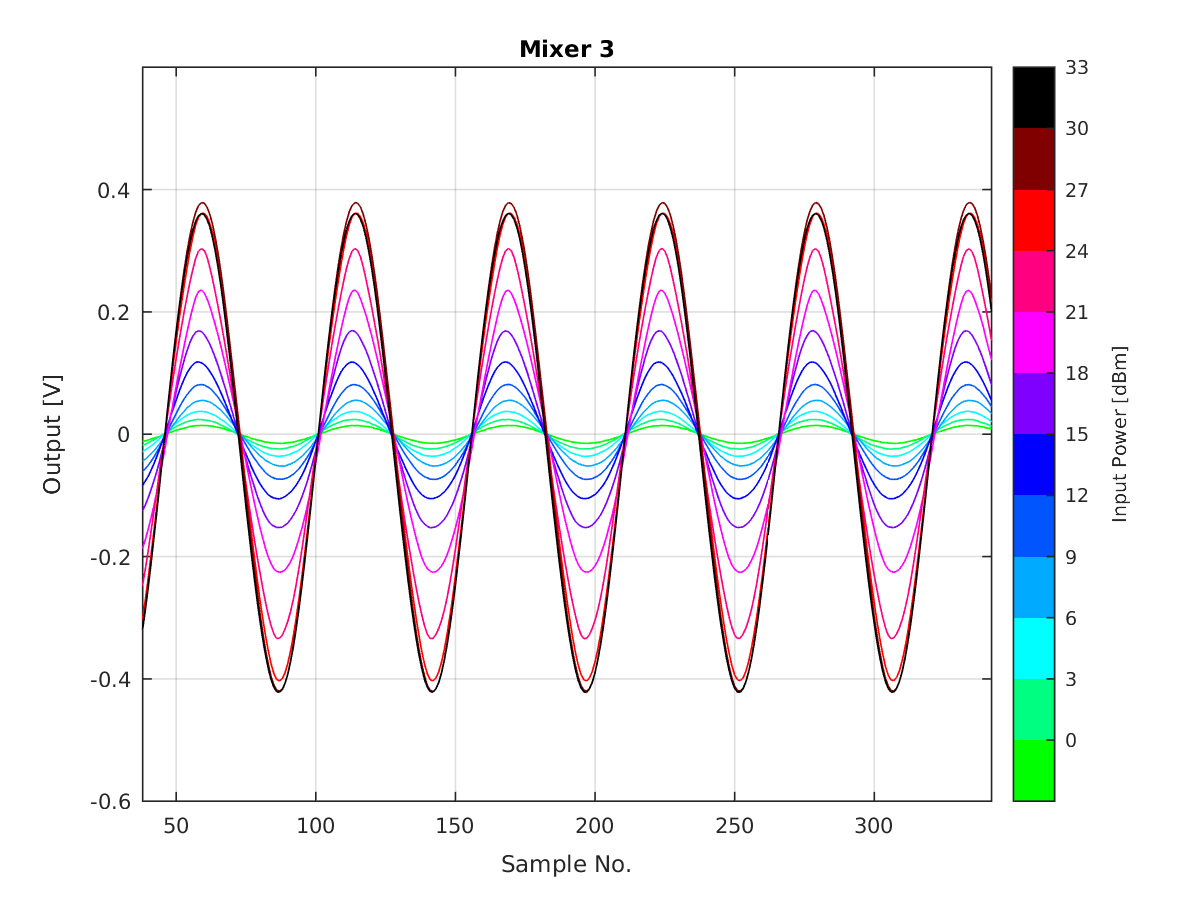
\includegraphics[width=0.9\textwidth]{Figures/phaseMons/Mixer3_AllPowerLevels}
  \caption{Response of Mixer 3 to signal generator input.}
  \label{f:sigGenAllMix3}
  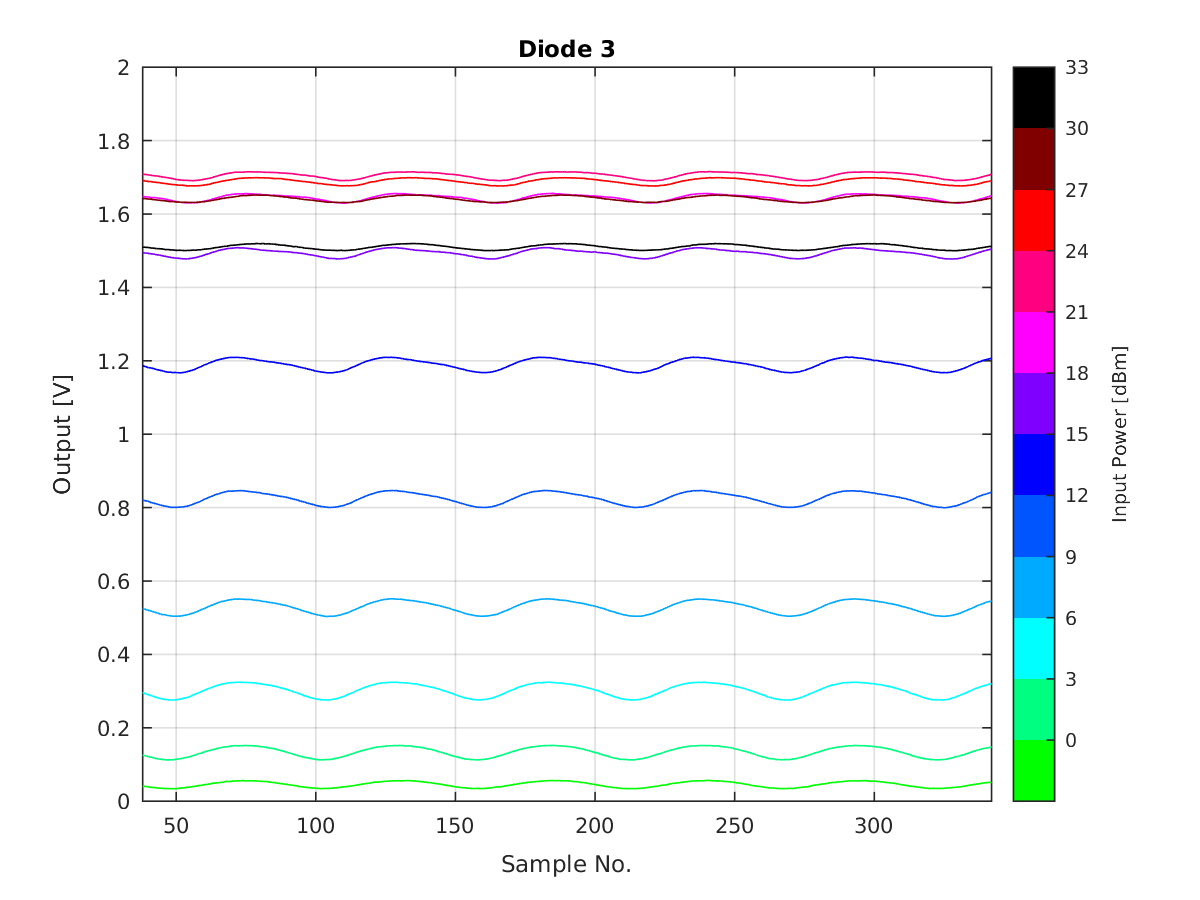
\includegraphics[width=0.9\textwidth]{Figures/phaseMons/Diode3_AllPowerLevels}
  \caption{Response of Diode 3 to signal generator input.}
  \label{f:sigGenAllDio3}
\end{figure}

\subsection{Mixer Performance}
\label{ss:sigGenMixer}

\subsubsection{Sinusoidal Characteristics}

Figure~\ref{f:mixersFit27dBm} shows fits to the response of all mixer outputs at an input power of 27~dBm, close to the typical input power from the beam signals when they are connected. Markers show the data points and the lines are sine fits to the data. The phase offset (displacement in peaks) between the output of each mixer holds no significance for the electronics performance. This is set only by the relative phase between the signal generator and the LO at the time the measurement was started. For normal operation with beam the LO phase shifters are changed to match the phasing of each set of electronics (Section~\ref{s:monCalibrations}).

The reconstruction of the phase from the mixer output depends on the mixer output being sinusoidal. In particular the maximum mixer output, or equivalently the gradient around zero mixer output (using the small angle approximation) is critical due to the dependence on the amplitude in Equation~\ref{e:phaseRecIdeal}. Each set of electronics has a different output amplitude due to slight differences in the LO power for each set of electronics and between the individual components used. At an input power of 27~dBm Mixer 1 has a higher peak output of 510~mV, compared to 410~mV and 380~mV for Mixer 2 and Mixer 3 respectively. 

Overall, the agreement between the actual mixer output and the sinusoidal fits at this input power is good. However, there is some distortion away from the ideal sine curve that is most visible around the maximum and minimum mixer output. Figure~\ref{f:mixersFitResid27dBm} shows the residuals between the mixer outputs and the sine fits across one half wavelength -- from maximum output to minimum output. In the figure the plotted residual is the difference between the fit and the data expressed in terms of an equivalent phase offset, \(\Delta \phi\), using:
\begin{equation}
\Delta \phi(t) = \arcsin\left(\frac{V_{MIXER}(t)-V_{FIT}(t)}{A}\right)
\end{equation}
Where \(V_{MIXER}(t)\) and \(V_{FIT}(t)\) are the mixer voltage and fitted voltage at sample \(t\) respectively, and \(A\) is the fitted mixer amplitude. On the falling slope between the peaks there is only a slight oscillation about the ideal sinusoidal behaviour. The deviation from ideal is at the level of \(0.25\pm0.03^\circ\) and \(0.30\pm0.04^\circ\) for the first and third mixers, with a slightly larger effect of \(0.45\pm0.04^\circ\) for the second mixer. This applies within \(\pm80^\circ\) of the zero crossing in the mixer output. Within \(\pm10^\circ\) of the maximum or minimum output the deviation from the sine fit rapidly increases, reaching several degrees for each mixer. For operation with the beam this means that the accuracy of the phase measurement cannot be guaranteed when the LO phase is set so that the mixer is giving close to its maximum or minimum output. This is also true for other reasons, as seen in Section~\ref{s:resolution}. The PFF system can only correct small offsets at the level of around \(\pm5^\circ\) (Section~\ref{ss:corrRange}), so the non-ideal response close to peak output is not an issue for the PFF performance.

\begin{figure}
  \centering
  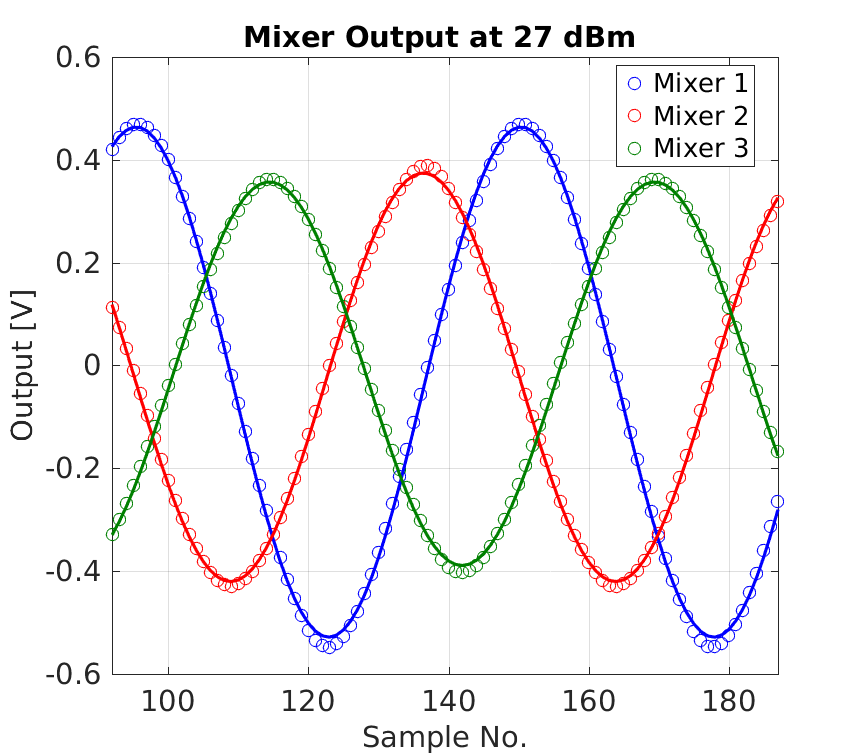
\includegraphics[width=0.9\textwidth]{Figures/phaseMons/mixersFit27dBm}
  \caption{Sinusoidal fit to mixer responses at 27~dBm input power.}
  \label{f:mixersFit27dBm}
\end{figure}

\begin{figure}
  \centering
  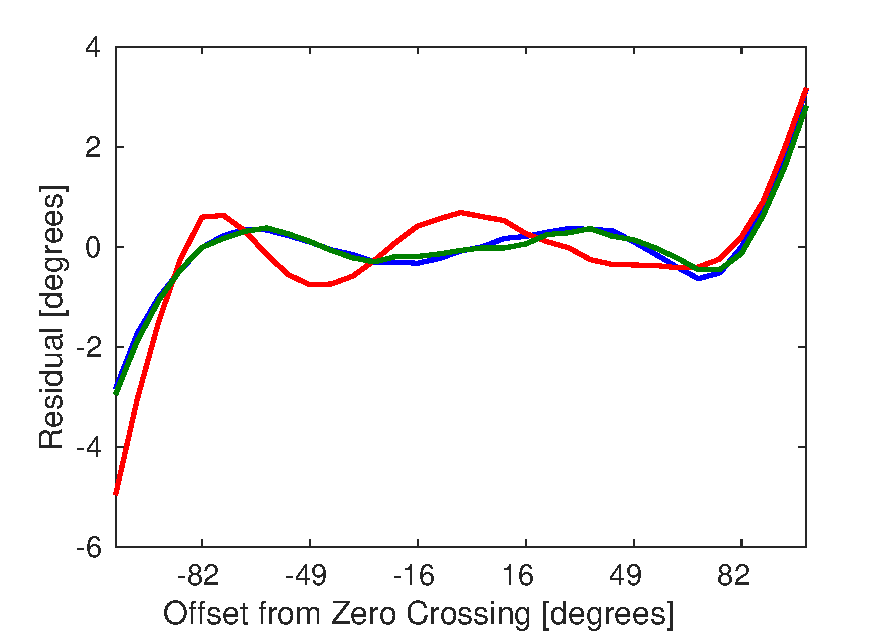
\includegraphics[width=0.9\textwidth]{Figures/phaseMons/mixersFitResid27dBm}
  \caption{Residuals to sinusoidal fit at 27dBm.[TODO: sample numbers don't relate to previous plots]}
  \label{f:mixersFitResid27dBm}
\end{figure}

However, for input powers in the range from 15--21~dBm the non-ideal characteristics of the mixers are larger. One example of this is shown in Figure~\ref{f:mixersFit18dBm}, at an input power of 18~dBm. If input powers in this range are used calibrations of the mixer response should normally be restricted to around the zero crossing so that the fitted amplitude gives the best approximation to the true behaviour for small phase offsets. 

\begin{figure}
  \centering
  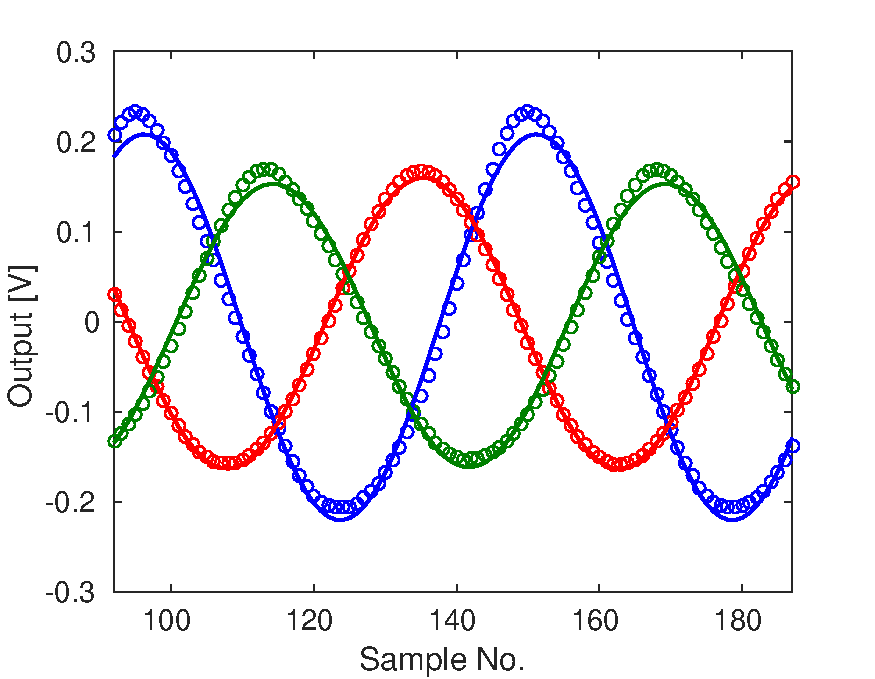
\includegraphics[width=0.9\textwidth]{Figures/phaseMons/mixersFit18dBm}
  \caption{Sinusoidal fit to mixer responses at 18~dBm input power.}
  \label{f:mixersFit18dBm}
\end{figure}

\subsubsection{Dependence on Input Power}

The mixer output is expected to linearly depend on the input voltage and the diode on the square of the input voltage. Both these dependencies must hold in order to use Equation~\ref{e:phaseRecIdeal} and obtain a phase measurement that does not depend on the input voltage to the electronics (therefore making the calculated phase insensitive to any possible variations in power along the pulse from the beam signal, for example). For these measurements the input voltage can be calculated using the known input power and 50~\(\Omega\) impedance of the electronics.

Figure~\ref{f:LinFitMixerVsVolts} shows the dependence of the mixer output amplitudes on the input voltage. As seen previously the first mixer gives a larger output than the other two mixers. The 2nd and 3rd mixers give a similar response up to an input voltage of 3.5~V (24~dBm). Dashed lines in the figure show a linear fit to the mixer output restricted to the range between 0.45~V and 1.75~V (6~dBm to 18~dBm) in each case, as marked by the vertical black lines. All three mixers give a linear response up to an input voltage of around 3~V (23~dBm), after which the effects of saturation begin to appear. By an input voltage of 5~V (27~dBm) the first and third mixers are almost fully saturated with almost no remaining power dependence in the output. The second mixer begins to enter saturation at the same voltage as the other two mixers but retains a strong power dependence up to a higher input voltage of 7~V (30~dBm).

\begin{figure}
  \centering
  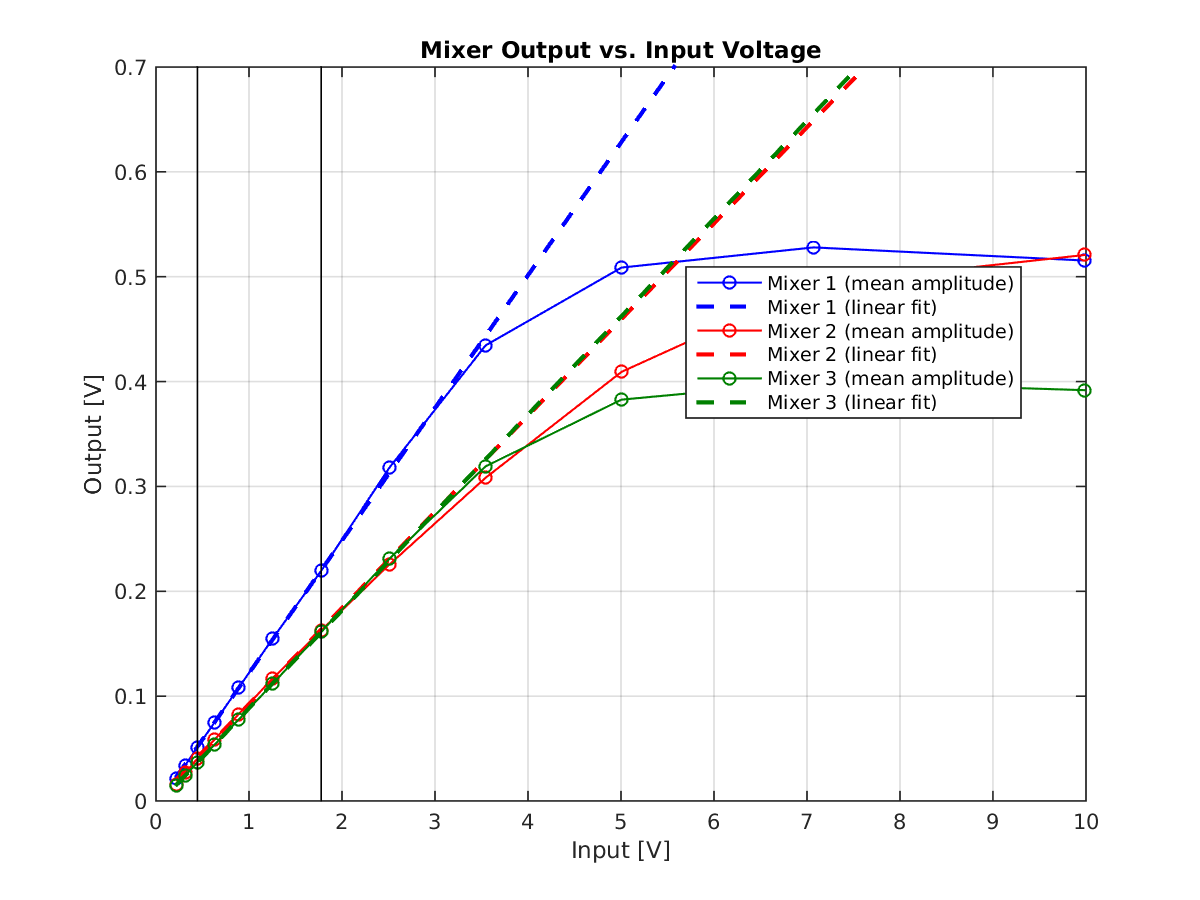
\includegraphics[width=0.9\textwidth]{Figures/phaseMons/LinFitMixerVsVolts}
  \caption{Linear fit to mixer output voltage vs. input voltage.}
  \label{f:LinFitMixerVsVolts}
\end{figure}


\subsubsection{Asymmetry in Output}

One final interesting property of the mixers is that the output is not symmetric about zero, in other words the maximum output voltage is different to the absolute value of the minimum output voltage. This is perhaps most visible looking back to the Mixer~1 output at all power levels in Figure~\ref{f:sigGenAllMix1}, where the maximum output is around \(+0.45~V\) but the minimum output is around \(-0.55~V\).

Figure~\ref{f:MixerVsVolts} shows how the mixer amplitude at maximum and minimum output varies with the input voltage. Mixer~1 asymmetry is largest for Mixer~1 and smallest for Mixer~3. The effect appears to increase in magnitude with the input voltage, with the \(\sim100\)~mV difference mentioned previously for Mixer~1 at an input of 10~V, but differences of only several mV at low input powers. For each mixer the amplitude at maximum output is larger for input voltages up to 2.5~V (21~dBm). Above 2.5~V input voltage this flips, with the minimum mixer amplitude being larger than the maximum amplitude.

\begin{figure}
  \centering
  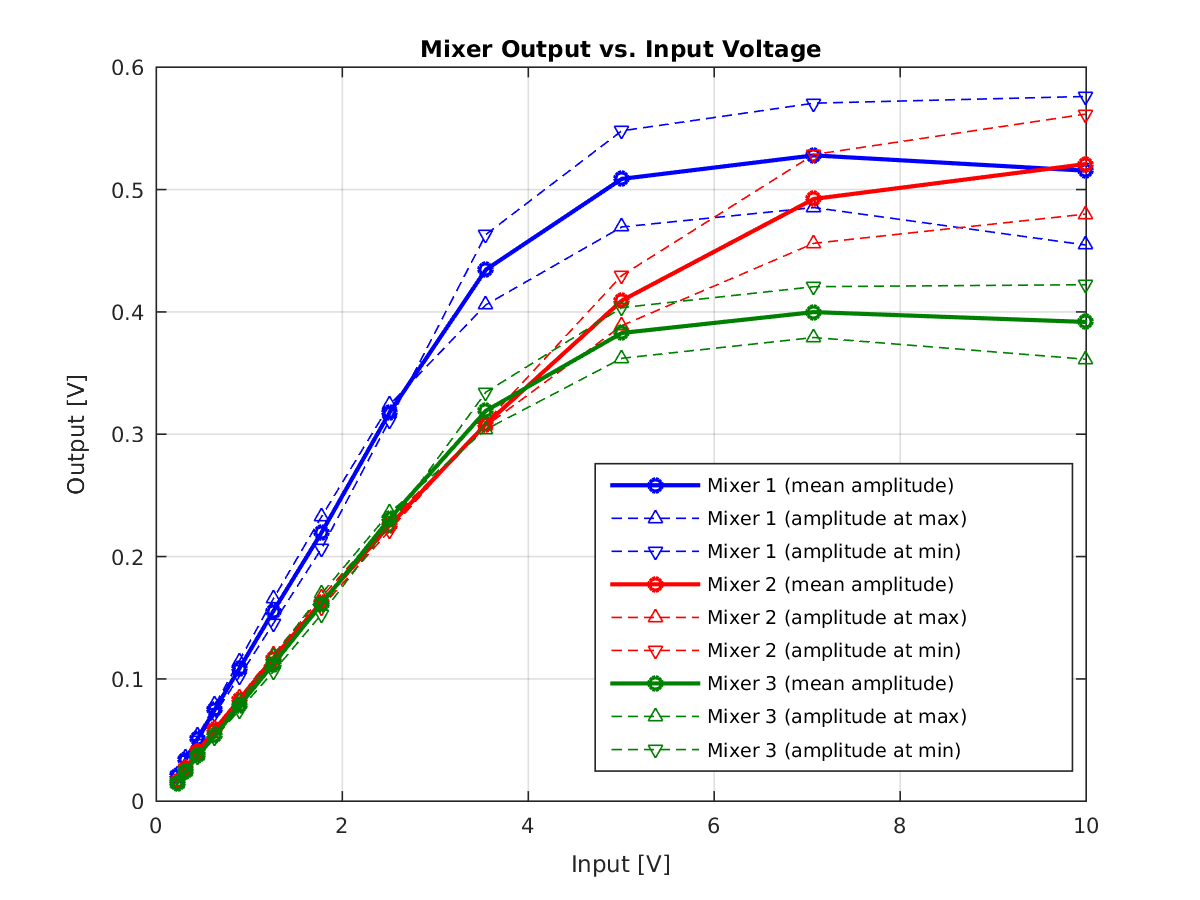
\includegraphics[width=0.9\textwidth]{Figures/phaseMons/MixerVsVolts}
  \caption{Mixer output voltage vs. input voltage.}
  \label{f:MixerVsVolts}
\end{figure}

For input voltages between 0.45~V and 1.25~V (6~dBm to 15~dBm) the mixer asymmetry has an approximate quadratic dependence on the input voltage, as shown in Figure~\ref{f:MixerAsymmetryVsVolts}. Outside this range there is no simple relationship that can explain the dependence of the asymmetry on the input voltage. One explanation for the asymmetry in the mixer outputs is cross-talk coming from the diode signals. Above 15~dBm the diodes enter saturation, as discussed in the next section, which may explain why the quadratic fit to the mixer asymmetry is only valid at power levels up to this value. 

\begin{figure}
  \centering
  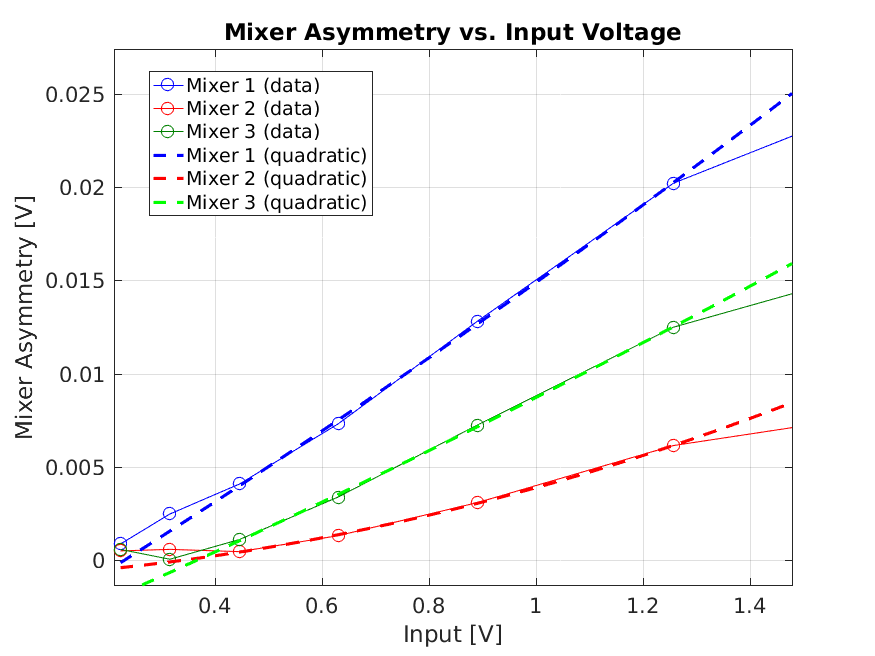
\includegraphics[width=0.9\textwidth]{Figures/phaseMons/MixerAsymmetryVsVolts}
  \caption{Relative amplitude vs. input power of cross-talk on the mixer from the diode.}
  \label{f:MixerAsymmetryVsVolts}
\end{figure}

Taking the power dependent asymmetry in to account the actual mixer response can be modified from Equation~\ref{e:mixOutSameFreq} to become:
\begin{equation}
\mathrm{Mixer}(t) = m_1A(t)\sin[\phi(t)] + m_2A(t)^2 + m_3A(t) + m_4
\label{e:actualMixerResponse}
\end{equation}
Where \(A(t)\) is the input voltage at time \(t\), and \(m_1\), \(m_2\), \(m_3\), and \(m_4\) are calibration constants.

\subsection{Diode Performance}
\label{ss:sigGenDiode}

\subsubsection{Dependence on Input Power}

The dependence of the three diode outputs on the input power is shown in Figure~\ref{f:SqrtDiodeVsVolts}, with the square root of the diode output plotted rather than the diode directly as this is the expected linear relationship. Immediately it is apparent that the diode signals saturate at much lower input voltages than the mixer signals. All three diodes are almost fully saturated at an input of 2~V (20~dBm), with the effects of saturation already beginning to appear above 1.25~V (15~dBm). Figure~\ref{f:LinFitSqrtDiodeVsVolts} shows a linear fit to the square root of the diode, using the range of input voltages between 0.45~V and 1.25~V (6--15~dBm). Even below saturation the response of sqrt(Diode) is not well approximated by a linear dependence as desired. However, in the range from 0.30~V 1.25~V (3~dBm to 15~dBm) a quadratic fit to the diode output directly (not sqrt(Diode)) does give a good approximation to the true dependence of the diodes on the input voltage. This is shown in Figure~\ref{f:QuadFitDiodeVsVolts}.

\begin{figure}
  \centering
  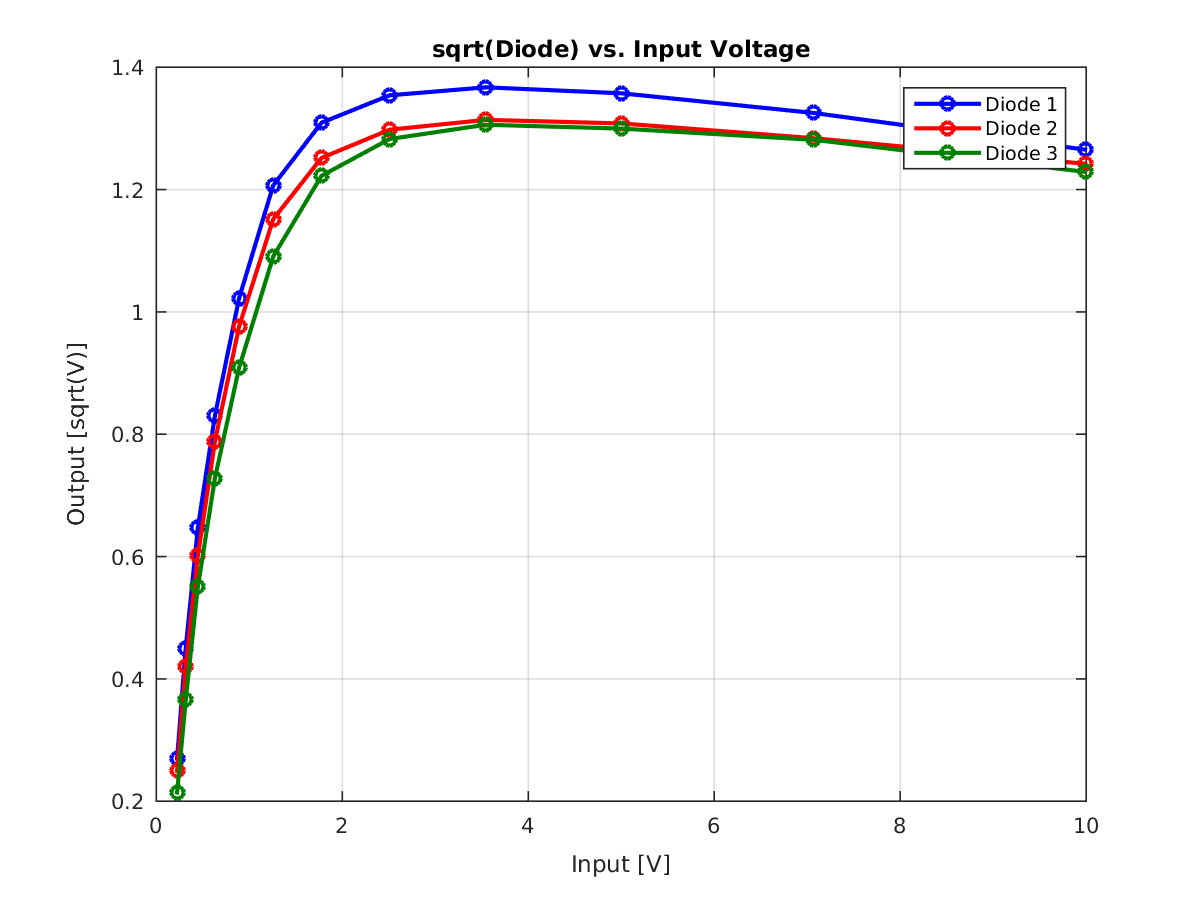
\includegraphics[width=0.9\textwidth]{Figures/phaseMons/SqrtDiodeVsVolts}
  \caption{sqrt(Diode) vs. input voltage.}
  \label{f:SqrtDiodeVsVolts}
\end{figure}

\begin{figure}
  \centering
  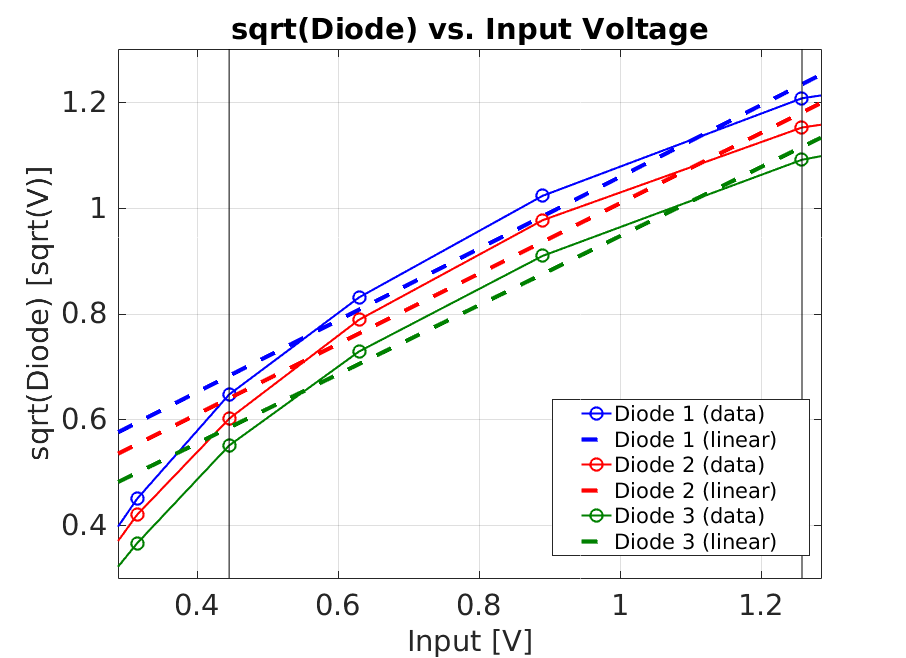
\includegraphics[width=0.9\textwidth]{Figures/phaseMons/LinFitSqrtDiodeVsVolts}
  \caption{Linear fits to sqrt(Diode) vs. input voltage.}
  \label{f:LinFitSqrtDiodeVsVolts}
  \centering
  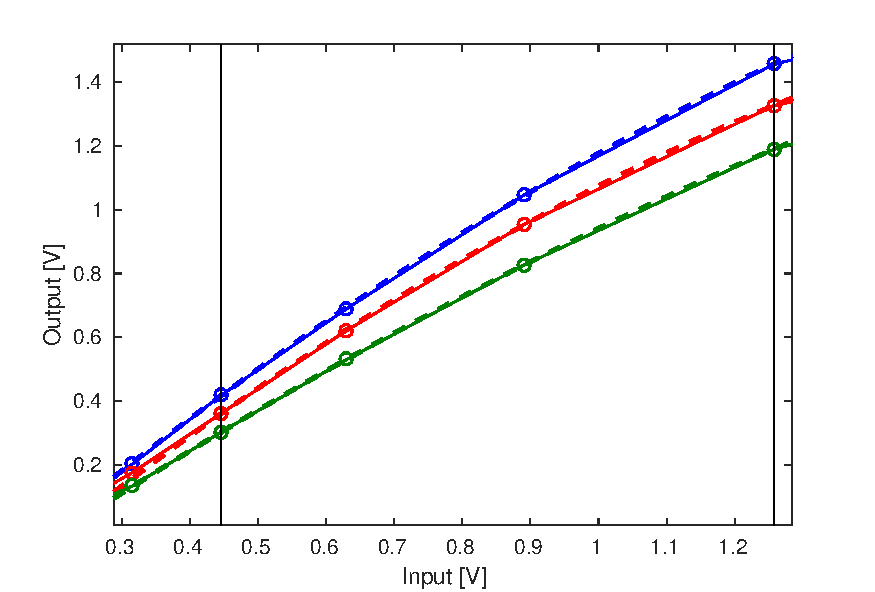
\includegraphics[width=0.9\textwidth]{Figures/phaseMons/QuadFitDiodeVsVolts}
  \caption{Quadratic fits to Diode vs. input voltage.}
  \label{f:QuadFitDiodeVsVolts}
\end{figure}

\subsubsection{Cross-Talk}

As seen previously in Figures~\ref{f:sigGenAllDio1},~\ref{f:sigGenAllDio2}~and~\ref{f:sigGenAllDio3} the diode outputs show a sinusoidal oscillation. Like there is cross-talk from the diode on the mixer outputs, there is also cross-talk from the mixers on the diode outputs. Figure~\ref{f:Diode1_Power6} shows a sinusoidal fit to the cross-talk on Diode~1 at an input power of 6~dBm. It has the same characteristics as the mixer output, including the slight distortion away from ideal sinusoidal behaviour around the peaks. However, as the diodes enter saturation the oscillation is initially distorted, and then has a much smaller amplitude when the diode output is fully saturated. One example of this is shown for the Diode~1 output at 18~dBm in Figure~\ref{f:Diode1_Power18}. The peaks around the maximum output are clearly non-sinusoidal in this case.

\begin{figure}
  \centering
  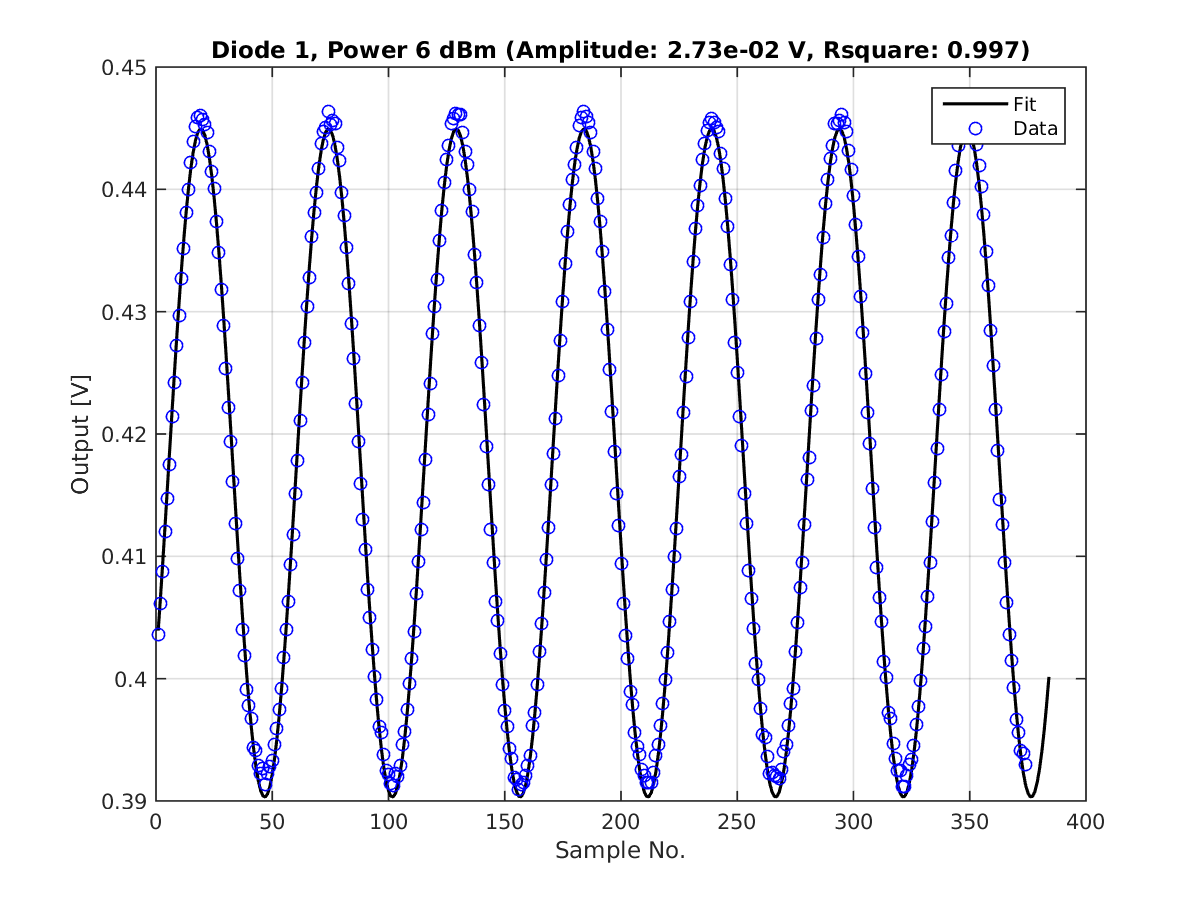
\includegraphics[width=0.9\textwidth]{Figures/phaseMons/Diode1_Power6}
  \caption{Sinusoidal fit to cross-talk on diode at 6~dBm input power.}
  \label{f:Diode1_Power6}
\end{figure}

\begin{figure}
  \centering
  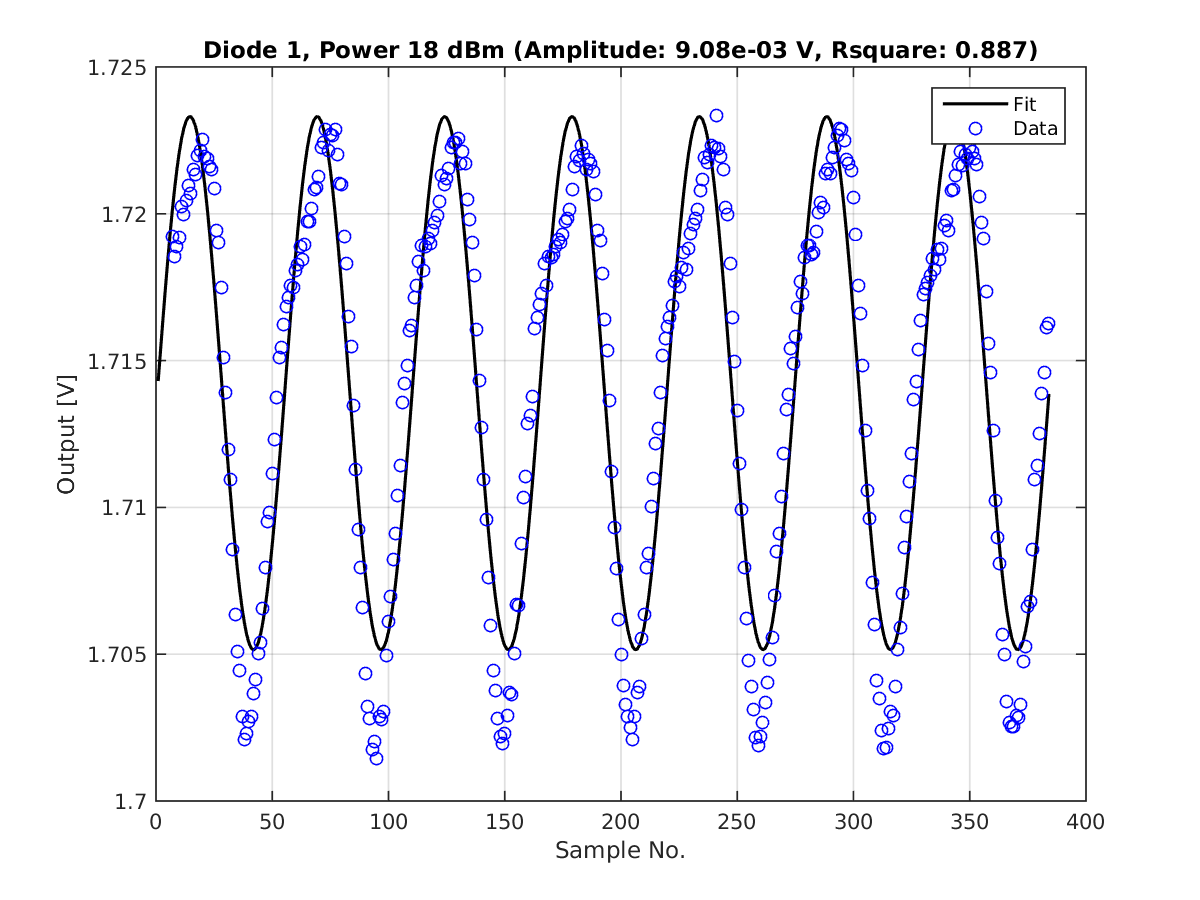
\includegraphics[width=0.9\textwidth]{Figures/phaseMons/Diode1_Power18}
  \caption{Sinusoidal fit to cross-talk on diode at 18~dBm input power.}
  \label{f:Diode1_Power18}
\end{figure}

Figure~\ref{f:RelativeDiodeXTalkVsPower} shows the dependence of the relative amplitude of the cross-talk on the input power. The relative amplitude of the cross-talk means the fitted amplitude of the sinusoidal oscillation on the diode divided by the mean diode output. Up until the diode outputs are fully saturated the relative amplitude of the cross-talk is around a factor two larger for the second diode. For example, at an input power of 12~dBm the relative cross-talk is at around the level of 30\% for the second diode, or 15\% for the first and third diode outputs. Up to input powers of 15~dBm the relative cross-talk is always above 10\%.

\begin{figure}
  \centering
  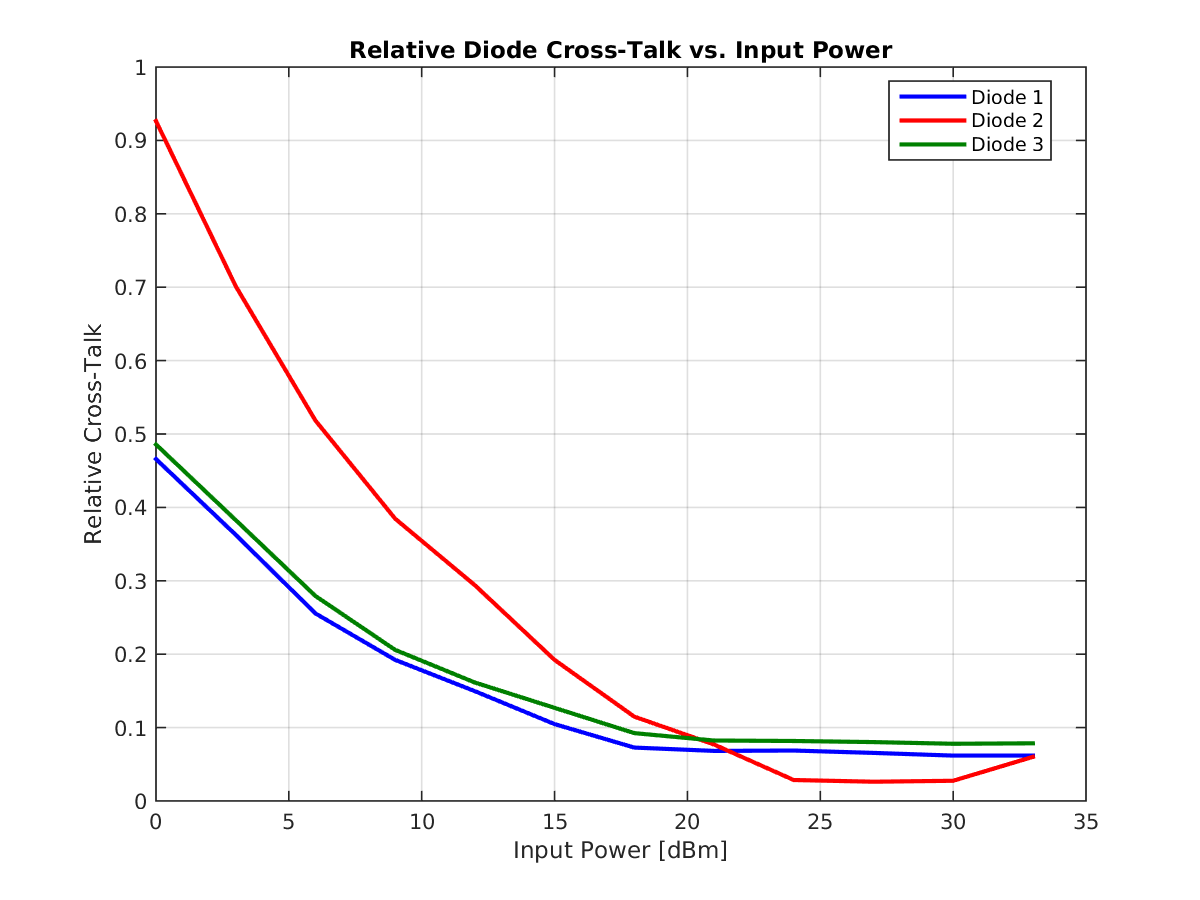
\includegraphics[width=0.9\textwidth]{Figures/phaseMons/RelativeDiodeXTalkVsPower}
  \caption{Dependence of the relative amplitude of cross-talk on the diode versus the input power.}
  \label{f:RelativeDiodeXTalkVsPower}
\end{figure}

Finally, Figure~\ref{f:PhaseDiodeVsMixer} compares the oscillation on the diode to the oscillation on the mixer. It can be seen that there is a phase shift between the two, which adds a further complication to the necessary phase reconstruction method. Taking in to account the actual characteristics of the diodes, including the cross-talk and quadratic dependence on the input power, the expected expression for the diode output from Equation~\ref{e:idealDiode} can be modified to:
\begin{equation}
\mathrm{Diode(t)} = d_1A(t)^2 + d_2A + d_3 + d_4A(t)\sin[\phi(t)+\delta]
\label{e:actualDiodeResponse}
\end{equation}
Where \(d_1\), \(d_2\), \(d_3\), \(d_4\) and \(\delta\) are calibration constants.

\begin{figure}
  \centering
  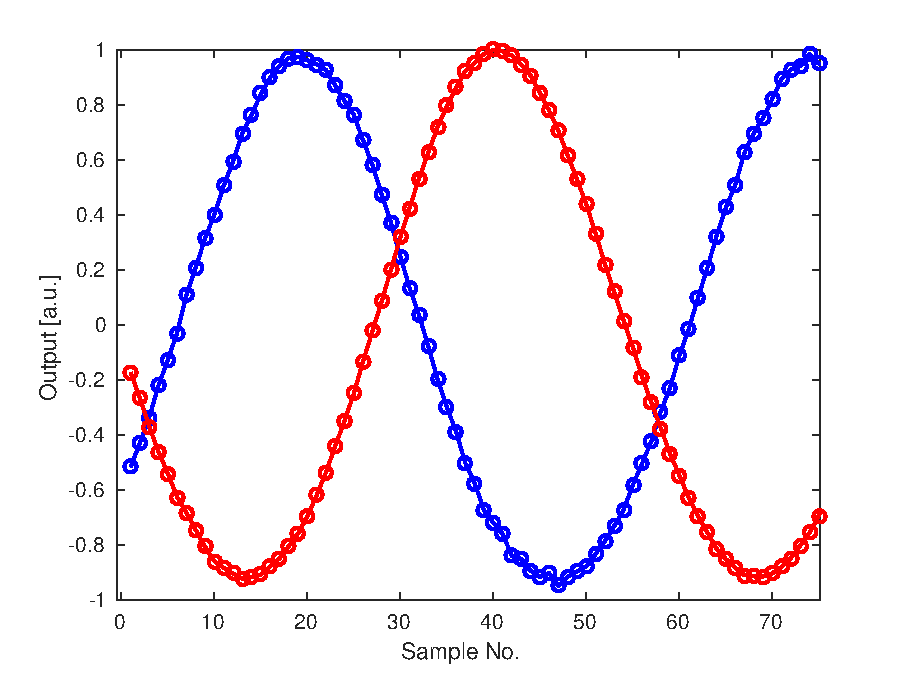
\includegraphics[width=0.9\textwidth]{Figures/phaseMons/PhaseDiodeVsMixer}
  \caption{Comparison of the oscillation on the mixer and the diode, showing a relative phase offset between the two.}
  \label{f:PhaseDiodeVsMixer}
\end{figure}

\subsection{Consequences for Normal Operation}
\label{ss:sigGenConsq}

The results of the signal generator tests have several consequences for the setup of the electronics and phase reconstruction during normal operation with the beam induced signals from the phase monitors. Firstly, in order to maximise the signal to noise ratio and yield the best possible resolution on the phase measurement the highest possible input power below saturation should normally be used. The degradation of the phase resolution with the input power is seen for beam based measurements in Section~[REF]. However, the diodes begin to enter saturation much earlier than the mixers, at around 15~dBm rather than 23~dBm. This means that in order to be able to use the diode measurement as part of the phase reconstruction the input power would have to be limited to below 15~dBm, 8~dBm lower than would be ideal for the mixer performance. There is no way to use different input powers for the mixers and diodes without a complete redesign of the electronics.

Secondly, the modifications that the cross-talk on the mixer and diode make to Equations~\ref{e:actualMixerResponse}~and~\ref{e:actualDiodeResponse} above makes the needed calculation to reconstruct the phase much more complex than the ideal case using Mixer/sqrt(Diode) in Equation~\ref{e:phaseRecIdeal}. In particular, the dependence of the diode output on \(\sin(\phi+\delta)\) means there is no simple expression that can be derived to create an input power independent phase measurement. An iterative process would have to be used to estimate the phase instead, converging towards the true diode output without cross-talk after each iteration using the estimated phase value. This may be possible in offline data analysis but would be difficult to implement in the PFF algorithm whilst still meeting latency requirements.

Due to these reasons, and with no possibility to make modifications to the electronics, the decision was eventually taken to not include the diode measurement in the phase reconstruction process. For operation with the beam this means making the assumption that the output power from the phase monitors is constant along the pulse, and that the jitter in the output power is small. This is a good approximation, as seen later in Section~[REF]. To reduce the sensitivity to any slow drifts in the output power due to changes in the beam conditions calibrations are taken at regular intervals between measurements.

With this treatment of the electronics outputs the phase is reconstructed as follows:
\begin{align}
&\mathrm{Mixer}(t) = A\sin[\phi(t)] + d \\
&\phi(t) = \arcsin\left(\frac{\mathrm{Mixer}(t)-d}{A}\right)
\label{e:phaseRecUsed}
\end{align}
Two calibration constants are needed -- \(A\) and \(d\). \(A\) is the fitted amplitude of the sinusoidal mixer output, and \(d\) is the asymmetry between the maximum and minimum mixer output. This is a simplified form of Equation~\ref{e:actualMixerResponse} given the assumption that the power is constant. In reality both \(A\) and \(d\) have a power dependence.

As any variations in input power are not removed by this method there is a benefit to operating the mixer in a region where the power dependence of the output is reduced. The best phase resolution achieved to date has been achieved with input powers to the electronics in the range between 24.5~dBm and 27~dBm (as stated in [REF]), where the mixers have actually begun to enter saturation, as a result. Operating in this range also has the benefit of reducing the deviation from ideal sinusoidal behaviour at lower input powers as seen in Section~\ref{ss:sigGenMixer}.


\newsection{monCalibrations}{Calibrations}

\subsection{Procedure}
\label{ss:calProcedure}

\subsection{Single Sample Results}
\label{ss:calSingSamp}

\subsection{Multi-Sample Results}
\label{ss:calMultiSamp}

\newsection{digNoise}{Digitiser Noise}

\subsection{On FONT5 Board}
\label{ss:font5Noise}

\subsection{On SiS Digitiser}
\label{ss:sisNoise}

\newsection{shifters}{Phase Shifter Noise}

\subsection{Digital Phase Shifters}
\label{ss:digShiftNoise}

\begin{figure}
  \centering
  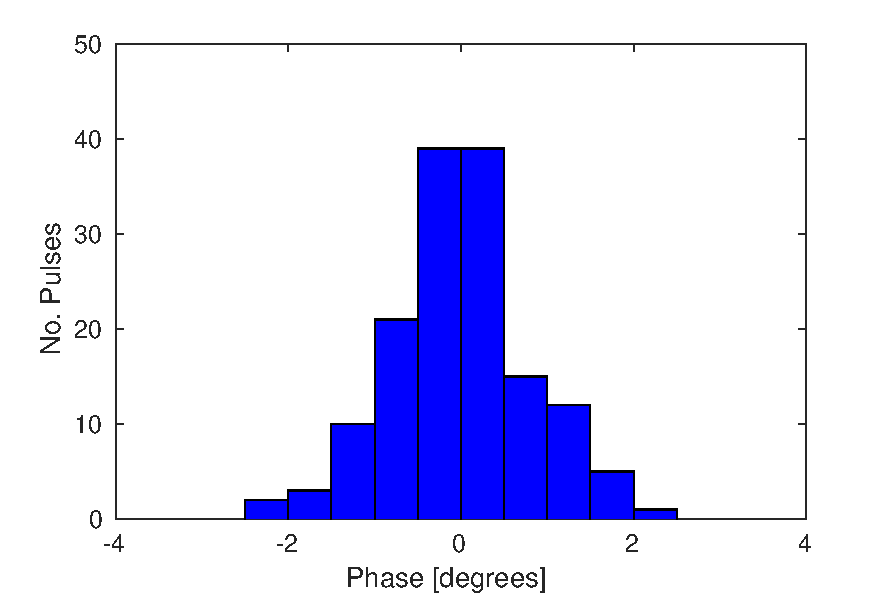
\includegraphics[width=0.9\textwidth]{Figures/phaseMons/PhMon_HistDig1}
  \caption{Dig shifter 1.}
  \label{f:PhMon_HistDig1}
\end{figure}

\begin{figure}
  \centering
  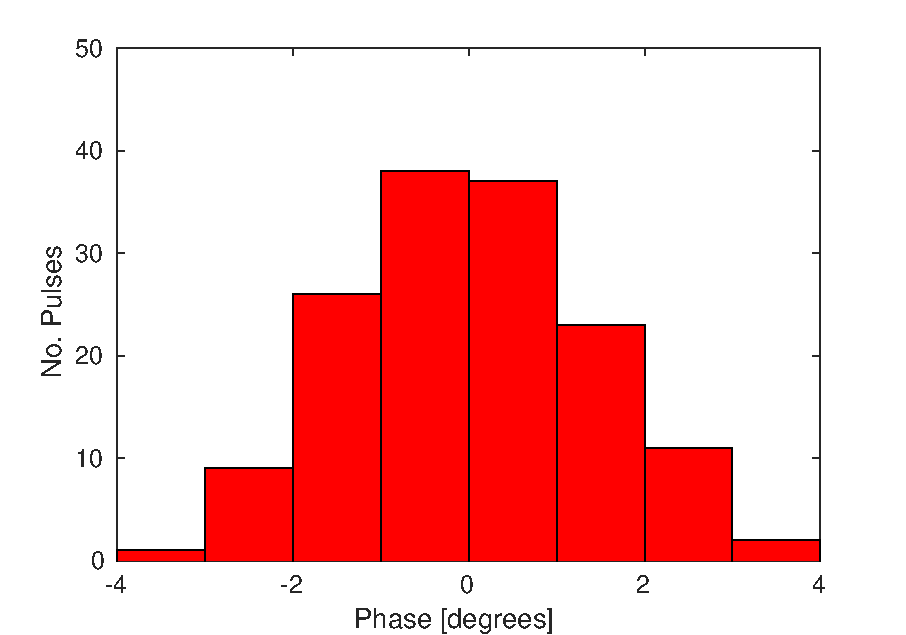
\includegraphics[width=0.9\textwidth]{Figures/phaseMons/PhMon_HistDig2}
  \caption{Dig shifter 2.}
  \label{f:PhMon_HistDig2}
\end{figure}

\begin{figure}
  \centering
  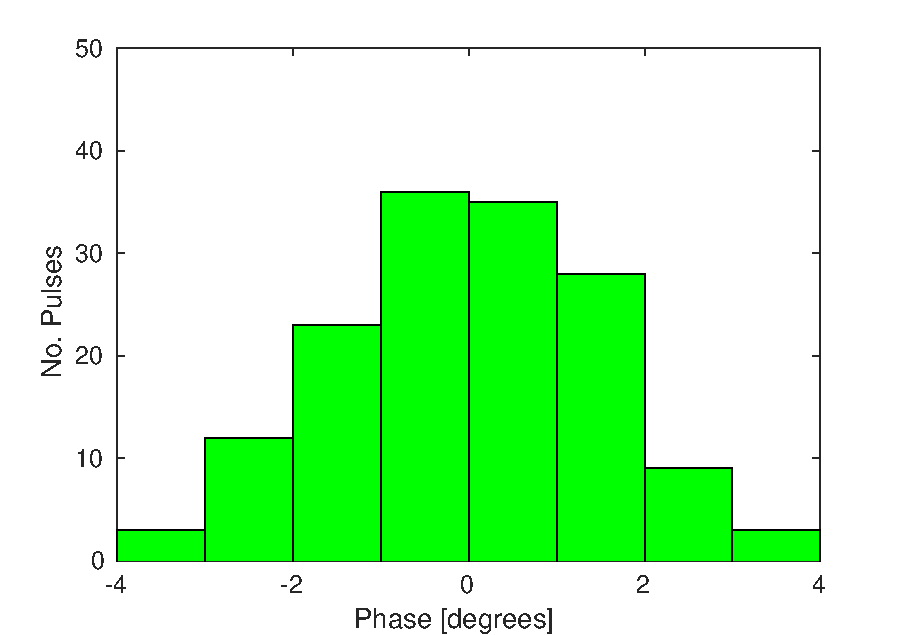
\includegraphics[width=0.9\textwidth]{Figures/phaseMons/PhMon_HistDig3}
  \caption{Dig shifter 3.}
  \label{f:PhMon_HistDig3}
\end{figure}

\subsection{Mechanical Phase Shifters}
\label{ss:mechShiftNoise}

\begin{figure}
  \centering
  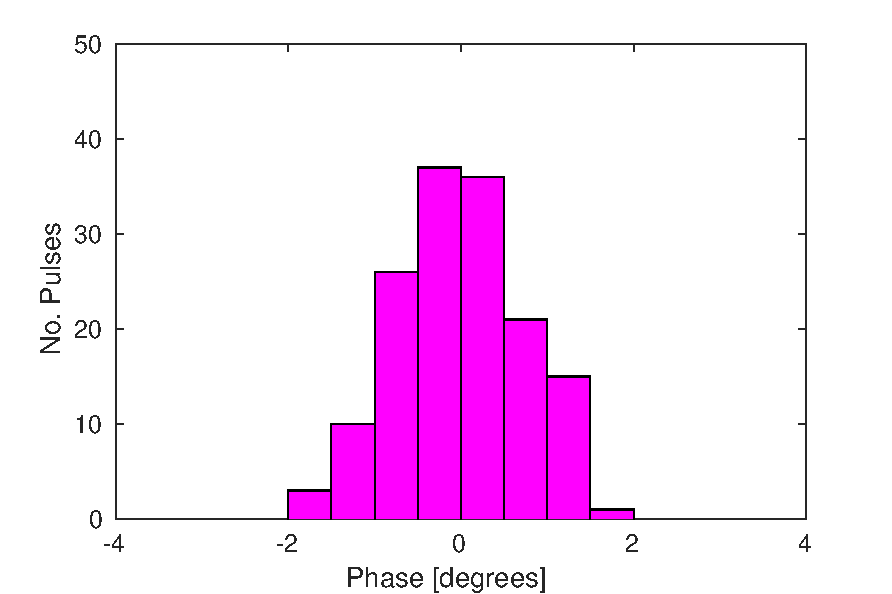
\includegraphics[width=0.9\textwidth]{Figures/phaseMons/PhMon_HistMech}
  \caption{Mech shifter.}
  \label{f:PhMon_HistMech}
\end{figure}

\newsection{resolution}{Resolution}

Single sample.

(Multi-sample)

Sample averaging.

Impact for phase correlations.

vs. shifter setting

\begin{figure}
  \centering
  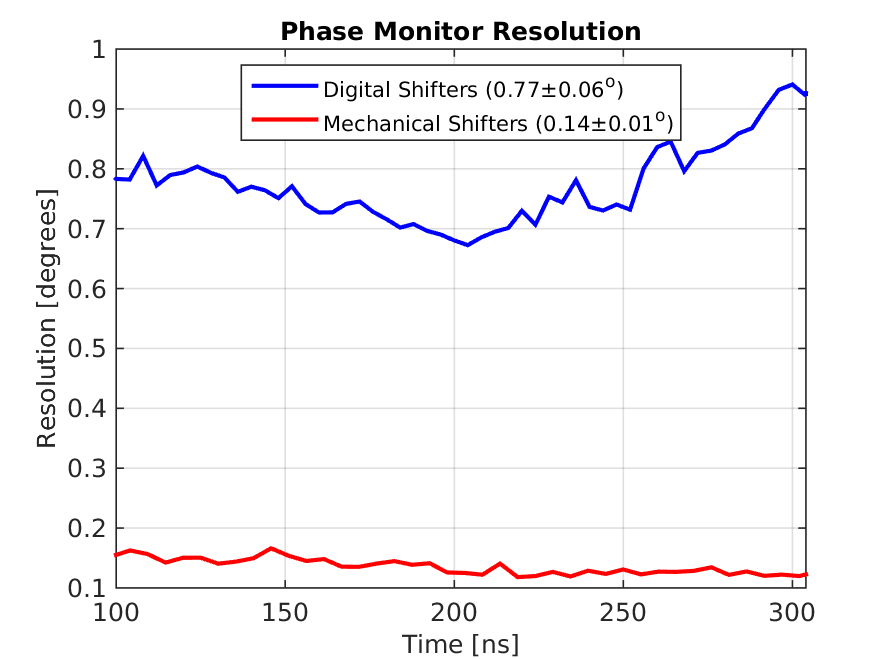
\includegraphics[width=0.9\textwidth]{Figures/phaseMons/PhMon_Resolution}
  \caption{Resolution.}
  \label{f:PhMon_Resolution}
\end{figure}

\newsection{monLinearity}{Linearity}

\newsection{monBandwidth}{Bandwidth}

\newsection{monPosition}{Dependence on Position}








